%++++++++++++++++++++++++++++++++++++++++
% Don't modify this section unless you know what you're doing!
\documentclass[letterpaper,11pt]{article}
\usepackage{natbib}
\bibliographystyle{unsrtnat}
\usepackage{tabularx} % extra features for tabular environment
\usepackage{amsmath}  % improve math presentation
\usepackage{amssymb}
\usepackage{graphicx} % takes care of graphic including machinery

\usepackage[margin=1in,letterpaper]{geometry} % decreases margins
%\usepackage{cite} % takes care of citations
\usepackage[final]{hyperref} % adds hyper links inside the generated pdf file
\hypersetup{
	colorlinks=true,       % false: boxed links; true: colored links
	linkcolor=blue,        % color of internal links
	citecolor=blue,        % color of links to bibliography
	filecolor=magenta,     % color of file links
	urlcolor=blue         
}

\DeclareMathOperator{\Tr}{Tr}
\DeclareMathOperator{\eff}{eff}
%+++++++++++++++++++++++++++++++++++++++
\begin{document}

\title{Final Report \\\textbf{Quantum Boltzmann Machine}}
\author{Yubin (Harvey) Hu}
\date{2021.12.13}
\maketitle

\begin{abstract}
In this report, we talk about a specific architecture for quantum machine learning (QML) called the Quantum Boltzmann Machine (QBM). Many QML architectures have been proposed, but the Quantum Boltzmann Machine is one of the few that has been experimentally realized on quantum hardware. We look into the setup of QBM, its training procedures, different variations, and experimental results on it. 
\end{abstract}

\section{Introduction}
Quantum computing promises greatly increased computing capabilities but harnessing these capabilities to perform useful tasks has proven hard except on a few selected problems (such as factorizing large numbers). Though finding useful things to do with quantum computing is hard, the fact remains that quantum computing produces atypical patterns that classical computers can not produce efficiently (\cite{NatureQML}). \par

Machine learning, on the other hand, is a rapidly developing area that requires great amount of compute. Increasingly, the effectiveness of modern machine learning models (especially in deep learning), cannot be predetermined theoretically, and must be determined via experiments. It seems that deeper and more computationally intensive models are more effective, though our understanding of why they are so effective is lacking (\cite{DeepLearning}). \par

Given the aforementioned properties of Quantum Computing and Machine Learning, it is an intriguing idea to somehow use the exponentially large amount of computational capabilities of quantum computing in building complex machine learning models of unknown usefulness, and then apply such models on real data to determine their effectiveness experimentally. \par

The challenge to developing this idea at the present time is that a general purpose quantum computer with low error rate and sufficient amount of qubits to perform machine learning tasks does not exist yet, and it may take a few decades for such a machine to become available. To perform a non-trivial machine learning task, thousands of tunable variables may be required, and current quantum computers are not large enough. Therefore an experimental approach is not feasible for most proposed quantum machine learning architectures. 

However, there is one specific architecture, the Quantum Boltzmann Machine (QBM), that can be experimentally realized on quantum annealers currently commercially available. In this report, we will examine how the Quantum Boltzmann Machine works what experiments has been done with it. 

\section{The Boltzmann Machine}

Inspired by the Ising model, the Boltzmann Machine (BM) is by nature closely related to quantum spins and physical processes. Here we introduce its design and how it can be used for machine learning. 

\subsection{Design}

A Boltzmann Machine utilizes the Boltzmann distribution to encode a machine learning model. The Boltzmann distribution give the probability of a system being in a specific micro-state $x$ as 
\begin{equation} \label{eq1}
P(x) \propto e ^ {- E(x)/k_B T}
\end{equation}
where $E(x)$ is the energy of this specific micro-state $x$, $k_B$ is the Boltzmann constant and $T$ is the temperature of the system. The inverse of the factor in this proportion relation is often called the partition function. It can be easily seen the partition function just the term on the right hand side summed over all possible micro-states. \par

\begin{figure}[h] 
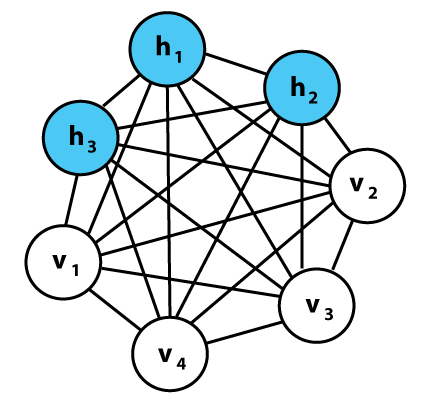
\includegraphics[width=0.3\textwidth]{BM.png}
\centering
\caption{Example of a Boltzmann Machine}
\label{fig1}
\end{figure}

The Boltzmann Machine is an undirected fully-connected graph (see an example in Figure~\ref{fig1}). Each vertex can take on value either zero or one, and each edge represent some interactions between two vertices. We use a vector $\vec{z} \in \mathbb{R}^N$, with each entry $z_i$ being zero or one, corresponding to vertex $i$, to represent the micro-state the system is in. The total energy of the system is defined as: \begin{equation}
E_{\vec{z}} = - \sum_a b_a z_a - \sum_{a,b} w_{ab} z_a z_b
\end{equation}
where $w_{ab}$'s are the interaction terms, and $b_a$'s are some fixed energy levels for being in the state ``1'' for each qubit (called a ``bias''). \par

\subsection{Supervised and unsupervised machine learning on BM} \label{MLonBM}

If we allow the system to evolve freely, there will be some probability distributions among all $2^{N}$ possible micro-states associated with each assignment of the $w$ and $b$ parameters. Matching this distribution to a target distribution of the data would allow us to generate more data like the given ones. If we further define some of the vertices as ``visible'' and some ``hidden'', we can perform feature extraction and auto-encoding (types of unsupervised learning) with the Boltzmann Machine. In \cite{ScienceRBM}, the authors built a Boltzmann Machine with significantly less hidden states than visible states, and trained the model. Later they were able to use the fewer hidden states to reproduce the data itself, effectively using the hidden states as ``primary features'' of the data. The authors also restricted parameters of the Boltzmann Machine to attain good efficiency, but since our focus is on QBM we will not discuss efficient methods to simulate the Boltzmann Distribution on classical machines. \textbf{Simply note that the Boltzmann Machine can carryout unsupervised machine learning tasks naturally, and that it has been shown useful for encoding image data.} \par

\begin{figure}[h] 
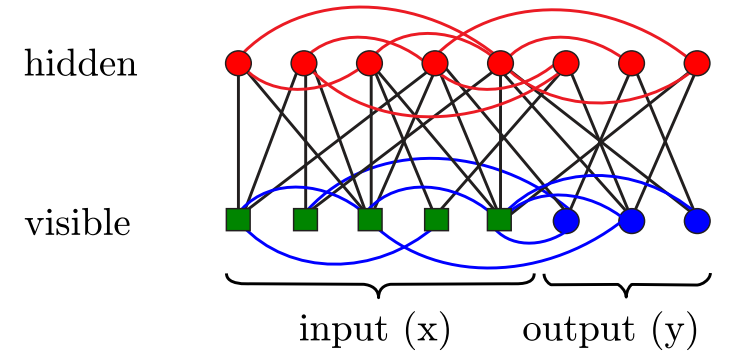
\includegraphics[width=0.6\textwidth]{FIG2.png}
\centering
\caption{Boltzmann Machine for Supervised Learning}
\label{fig2}
\end{figure}

If we further divide our visible vertices into ``input'' vertices and ``output'' vertices (see Figure~\ref{fig2}), we would be able to perform supervised machine learning tasks. We could either ``clamp'' the input vertices down to the given inputs and then train the network to generate the desired outputs, or we could treat the input output pair as a single piece of data and train the network to generate it. 

\subsection{Training}

To perform training, we need a gradient to give us a direction to change the parameters to. To get a gradient, we need to first define a loss function. We want to match the probability distribution given by BM over visible vertices $P_v$ with this distribution in the data $P_v^{data}$. Using the average negative log-likelihood loss function, we get:
\begin{equation} \label{eq3}
\mathcal{L} = - \sum_{\vec{v}} P_{\vec{v}}^{data} \log P_{\vec{v}}
\end{equation}
Plug in the Boltzmann Distribution from Eq.~\ref{eq1}, we get 
\begin{equation} \label{eq4}
\mathcal{L} = - \sum_{\vec{v}} P_{\vec{v}}^{data} \log \frac{\sum_{\vec{h}} e^{-E_{\vec{z}(\vec{h}, \vec{v})}}}{\sum_{\vec{h'}, \vec{v'}} e^{-E_{\vec{z}(\vec{h'}, \vec{v'})}}}
\end{equation}
where $\vec{z}(\vec{h}, \vec{v})$ is the total state with hidden state as $\vec{h}$ and visible state as $\vec{v}$. The gradient we are looking for is:
\begin{equation} \label{eq5}
\partial_{\theta} \mathcal{L} = \sum_{\vec{v}} P_{\vec{v}}^{data}\langle \partial_{\theta} E_{\vec{z}}\rangle_{\vec{v}} - \langle \partial_{\theta} E_{\vec{z}}\rangle := \overline{\langle \partial_{\theta} E_{\vec{z}}\rangle_{\vec{v}}} - \langle \partial_{\theta} E_{\vec{z}}\rangle
\end{equation}
where the $\langle ...\rangle_{\vec{v}}$ denotes the expectation for ``$...$'' according to the Boltzmann Distribution when we fix the visible nodes to $\vec{v}$. \par
With this equation, we can calculate the gradient via sampling if there's an efficient algorithm for sampling. By restricting the number of parameters, people have found such an algorithm and successfully trained restricted Boltzmann machines (BM without connections between nodes in the hidden layer). \cite{QBM}

\section{The Quantum Boltzmann Machine}
Next we talk about proposed architectures of a Quantum Boltzmann Machine. The QBM is capable of implementing universal quantum logic (\cite{NatureQML}). 

\subsection{Design}
Replace all the nodes that take on values zero or one in the classical Boltzmann Machine with qubits. The qubits are measurable in the z-axis. Now we can rewrite the Hamiltonian in the following form:
\begin{equation} \label{QH}
H = - \sum_a b_a {\sigma}_a^z - \sum_{a,b} w_{ab} {\sigma}_a^z {\sigma}_b^z
\end{equation}
where ${\sigma}_a^z$ is acting the ${\sigma}^z$ operator on the $a$'th qubit while not changing any other qubit. \par

Simply using this Hamiltonian we can make a quantum Boltzmann Machine with the same theoretical behavior as a classical one, but more efficient due to access to fast sampling using quantum hardware (\cite{QBM}). Though  polynomial time sampling algorithms on classical machines exists, it is reasonable to expect that for models with larger amount of hidden states, the quantum annealer hardware could allow faster gradient calculations than classical methods. \par

Alternatively, we could add another term to this Hamiltonian to make the model itself ``quantum.'' When talking about making a system ``quantum'', what we mean that the Hamiltonian would involve the ``non-observable'' axes, or having non-diagonal terms in the Hamiltonian. For example, adding some ${\sigma}^x$ terms:
\begin{equation} \label{QH2}
H = - \sum_a \Gamma_a {\sigma}_a^x - \sum_a b_a {\sigma}_a^z - \sum_{a,b} w_{ab} {\sigma}_a^z {\sigma}_b^z
\end{equation} 
where the $\Gamma$'s are some additional parameters. \par

In the following analysis we will use this second Hamiltonian, since setting the $\Gamma$'s to zero would give us the first Hamiltonian. As we will see, using this second Hamiltonian poses challenges in training. The authors who proposed this architecture did not find any good way to train the $\Gamma$ parameters, so they proposed to constrain all $\Gamma$'s to be the same and have this global $\Gamma$ value left as a ``hyper-parameter.'' More efficient training methods for QBM that utilizes quantum computing better may be an interesting area for future developments. \par

Since the procedures using a trainable QBM to do machine learning is the same as the procedures for classical Boltzmann Machines discussed in Section \ref{MLonBM}, we will now move on to discussing how to train a QBM.  

\subsection{Training a QBM}
First we need to adapt the Boltzmann Distribution for the quantum case. The Boltzmann Distribution of a system of qubits can be given as the following: If we define a partition function $Z = \Tr[e^{-H}]$, then we can define a density matrix of all the qubits as the following
\begin{equation}
\rho = Z^{-1} e^{-H}
\end{equation} \par

Then we know the probability $P_{\vec{v}} = \Tr [\Lambda_{\vec{v}} \rho]$, where $\Lambda_{\vec{v}}$ is a diagonal matrix with diagonal matrix as 1 if the corresponding node is visible and 0 if not. To calculate the gradient we get:

\begin{equation}
\partial_{\theta} \mathcal{L} = \sum_{\vec{v}} P_{\vec{v}}^{data} (\frac{ \Tr[\Lambda_{\vec{v}} \partial_{\theta} e ^ {-H}]}{\Tr[\Lambda_{\vec{v}} e ^ {-H}]} - \frac{\Tr[\partial_{\theta} e^{-H}]}{\Tr[e^{-H}]})
\end{equation}

Since $H$ and $\partial_{\theta} e^{-H}$ may not commute now, estimating the first term requires numerical estimations (details see \cite{QBM}) and cannot be efficiently calculated. \par

A workaround is developed in which an upper bound of the loss replaces the loss function itself, and allows for efficient gradient calculations. \par

Using the Golden Thompson inequality: for any Hermitian matrices A and B,
\begin{equation}
\Tr[e^A e^B] \geq \Tr[e^{A + B}]
\end{equation}
we have
\begin{equation}
\Tr[e^{-H} e^{\ln(\Gamma_{\vec{v}} + \epsilon)}] \geq \Tr[e^{-H + \ln(\Gamma_{\vec{v}} + \epsilon)}]
\end{equation}, where $\epsilon$ is a small number. 
Taking $\epsilon$ to zero gives $\Tr[e^{-H + \ln(\Gamma_{\vec{v}} + \epsilon)}] \rightarrow \Tr[e^{-H_{\vec{v}}}]$ where $H_{\vec{v}} = \langle \vec{v} | H | \vec{v}\rangle$ is the clamped Hamiltonian. 
This gives us an approximate loss function 
\begin{equation}
\mathcal{L} \leq \tilde{\mathcal{L}} := -\sum_{\vec{v}} P_v^{data} \log{\frac{\Tr[e^{-H_{\vec{v}}}]}{\Tr[e^{-H}]}}
\end{equation} 
and calculating the gradient of this function gives us
\begin{equation}
\partial_{\theta} \tilde{\mathcal{L}} = \overline{\langle \partial_{\theta} H_{\vec{v}}\rangle_{\vec{v}}} - \langle \partial_{\theta} H\rangle
\end{equation}
where
\begin{equation}
\overline{\langle ... \rangle_{\vec{v}}} := \sum_{\vec{v}} P_{\vec{v}}^{data} \frac{\Tr[e^{-H} ...]}{\Tr[e^{-H}]}
\end{equation}

One thing to notice here is that this approximate loss cannot be used to optimize for $\Gamma$'s, because the gradients vanishes due to our approximation (Math see \cite{QBM}). This means that we cannot use perform gradient descent on the $\Gamma$ parameters. The author for this proposal suggested that they should be all restricted to take on the same value, and then this same value can be left as a hyper-parameter for manual adjustment. It's not the best solution but the QBM does outperform other BM on some of the toy models \cite{QBM} proposed. It is then reasonable to assume that the QBM captures some more complex relations between hidden and visible variables because of the $\Gamma$ variables, though a better way to train them is still yet to be discovered. \par

It is also possible to simply set all $\Gamma$ terms to zero, in which case the QBM would become a BM on quantum hardware. \par

To perform supervised learning on QBM, we do not need to assign any qubit to the input. Suppose we have input $\vec{x}$ and output $\vec{y}$. We can change the biases of every qubit in the system to incorporate the input. The new Hamiltonian would become:
\begin{equation}
H_{\vec{x}} = - \sum_a [\Gamma_a \sigma_a^x + b_a^{\eff} (\vec{x})] - \sum_{a,b} w_{ab} \sigma_a^z \sigma_b^z
\end{equation} and 
\begin{equation}
b_a^{\eff} (\vec{x}) = b_a + \sum_{\mu} w_{a \mu} x_{\mu}
\end{equation}, where $a$, $b$ range over all physical qubits and $\mu$ range over all the input bits in $\vec{x}$. \par

By now we have finished discussing how to train a QBM and how to use QBM to perform supervised or unsupervised learning tasks. 

More recently, \cite{Zoufal_2021} has proposed a variational way to implement QBM on gate-based quantum computers. Their algorithm is based on imaginary time evolution and McLachlan's variational principle on gate based quantum computers introduced in \cite{VariationalQS}. With this implementation, analytical gradients for generic QBMs with long range interactions are possible to calculate. However, the hardware that can support this architecture is not available yet. It may become available in the short-term (according to \cite{Zoufal_2021}). 

\subsection{Experimental Results}

At this time, there's still limited experimental results on QBM. In \cite{reinforcement}, they constructed a ``Deep Restricted Quantum Boltzmann Machine (DRQBM)'', which has a similar graph structure (but different interaction patterns) to a typical multilayered neural network. The DRQBM has multiple layers of hidden nodes (thus ``deep''), each connected to nodes to other layers and the visible layer, but not to nodes in the same layer (thus ``restricted''). They used this DRQBM on a typical reinforcement learning task where the it seems to have a small advantage over a classical BM of the same structure. 

Some very recent research include the experiments done in \cite{TrainingRQBM} and in \cite{cyber}, where they trained QBM with 64 visible and 64 hidden nodes. The tasks were image reconstruction and classifying cyber-security data. In both cases, no advantage of the QBM over classical methods were found, but there are many details to be optimized for the QBM and more experiments are still warranted. Particularly, in \cite{TrainingRQBM}, it is demonstrated that noise in the hardware is currently limiting the performance of the QBM, as two versions of QBM trained on hardware with different noise levels are compared. \par


\section{Conclusion}
We have reviewed the design of the Quantum Boltzmann Machine and how it could be used for machine learning tasks. Theory behind the QBM still has room for development but it's one of the rare instances of quantum machine learning where experimental observations could happen as theories are being developed concurrently. \par

It would be very interesting to see more experiments done on the QBM for different tasks, as well has hardware improvements like noise reductions. Possible future directions include better gradient calculations, alternative ways to define interactions between qubits, and new ways to encode new problems in the Hamiltonian of the QBM. 



\bibliography{references}




\end{document}
